\documentclass{article}
\usepackage[margin=0.8in]{geometry}
\usepackage{amsmath}
\usepackage{ctex}
\usepackage{siunitx}
\usepackage{multirow}
\usepackage{bigstrut}
\usepackage{graphicx} 
\usepackage{hyperref}
\title{直流电源特性实验报告}
\author{姓名:宋建宏\,\, 学号:PB21020677\,\, 班级:203院22级5班\\ 日期:2023年4月28日}
\date{}

\begin{document}
\maketitle
\section*{实验目的}
测量交流电流滤波后所得直流电源的输出功率和纹波系数随负载的变化,通过等效电路和补偿法来测量电池的开路电压和短路电流并求其内阻。

\section*{实验原理}


\subsection*{波纹系数}
直流稳压电源直流稳定量中不可避免地带
有一些交流成分,这种叠加在直流稳定量上的交流分量就称之为纹波。纹波系数是指负载上交流电压的有效值与直流电压之比
\begin{equation*}
    \text{波纹系数}K_u=\frac{\text{交流电压有效值}}{\text{直流电压}}\times 100\%
\end{equation*}
是表征直流电源品质的一个重要参数。除了与整流滤波电路品质有关之外,与外电路负载关系也很大。

\subsection*{电源开路电压和短路电流}
开路电压是指电源在断路时的输出电压值,短路电流是指外电源短路时的最大电
流。由于电压表的内阻不是无穷大,而电流表内阻也不可能为零,而且电源短路的时候容易烧毁电源,因此不能
直接用电压表或电流表测量电源的开路电压和短路电流。因此采用等效电路或补偿法来进行测量,电路图如下图
所示。

\begin{figure}[htbp]
    \centering
    \includegraphics*[scale=1]{dl.png}
\end{figure}

\section*{测量记录与数据处理}
\subsection*{不同负载下纹波系数和功率的测量}如下表
% Table generated by Excel2LaTeX from sheet 'Sheet1'
\begin{table}[p]
    \centering
    \begin{tabular}{|r|r|r|r|r|r|r|r|r|r|}
        \hline
        \multicolumn{5}{|c|}{pi型RC电路} & \multicolumn{5}{c|}{单电容电路} \bigstrut                                                                                                                                                                                                                                         \\
        \hline
        \multicolumn{1}{|l|}{负载}      & \multicolumn{1}{l|}{交流电压}            & \multicolumn{1}{l|}{直流电压} & \multicolumn{1}{l|}{负载功率} & \multicolumn{1}{l|}{纹波系数} & \multicolumn{1}{l|}{负载} & \multicolumn{1}{l|}{交流电压} & \multicolumn{1}{l|}{直流电压} & \multicolumn{1}{l|}{负载功率} & \multicolumn{1}{l|}{纹波系数} \bigstrut \\
        (/$\Omega$)                   & (/mV)                                & (/mV )                    & (/mW)                     &                           & (/$\Omega$)             & (/mV)                     & (/V )                     & (/mW)                     & \bigstrut                           \\
        \hline
        20                            & 9.673                                & 51.37                     & 0.1319                    & 18.83\%                   & 20                      & 241.5                     & 0.5371                    & 14.42                    & 44.96\% \bigstrut                  \\
        \hline
        30                            & 14.08                                & 76.56                     & 0.1954                    & 18.39\%                   & 30                      & 263.8                     & 0.7254                    & 17.54                    & 36.36\% \bigstrut                  \\
        \hline
        40                            & 18.15                                & 101.3                     & 0.2565                    & 18.31\%                   & 40                      & 268.9                     & 0.8836                    & 19.52                    & 30.43\% \bigstrut                  \\
        \hline
        50                            & 23.02                                & 125.9                     & 0.3170                    & 18.28\%                   & 50                      & 266.8                     & 1.019                     & 20.76                    & 26.18\% \bigstrut                  \\
        \hline
        70                            & 28.60                                & 173.6                     & 0.4305                    & 16.48\%                   & 60                      & 261.5                     & 1.137                     & 21.54                    & 22.99\% \bigstrut                  \\
        \hline
        100                           & 36.30                                & 242.7                     & 0.5890                    & 14.96\%                   & 70                      & 255.0                     & 1.224                     & 21.40                    & 20.83\% \bigstrut                  \\
        \hline
        130                           & 41.85                                & 308.8                     & 0.7335                    & 13.55\%                   & 80                      & 247.9                     & 1.334                     & 22.24                    & 18.58\% \bigstrut                  \\
        \hline
        160                           & 45.82                                & 372.3                     & 0.8663                    & 12.31\%                   & 90                      & 240.7                     & 1.417                     & 22.31                    & 16.98\% \bigstrut                  \\
        \hline
        200                           & 49.36                                & 453.2                     & 1.027                     & 10.89\%                   & 100                     & 233.6                     & 1.492                     & 22.26                    & 15.65\% \bigstrut                  \\
        \hline
        250                           & 51.96                                & 548.6                     & 1.204                     & 9.471\%                   & 120                     & 220.3                     & 1.624                     & 21.97                    & 13.56\% \bigstrut                  \\
        \hline
        300                           & 52.23                                & 637.9                     & 1.356                     & 8.188\%                   & 140                     & 208.1                     & 1.735                     & 21.50                    & 11.99\% \bigstrut                  \\
        \hline
        350                           & 53.74                                & 722.0                     & 1.489                     & 7.443\%                   & 160                     & 197.2                     & 1.831                     & 20.95                    & 10.77\% \bigstrut                  \\
        \hline
        400                           & 53.76                                & 801.2                     & 1.605                     & 6.710\%                   & 180                     & 187.4                     & 1.915                     & 20.37                    & 9.786\% \bigstrut                   \\
        \hline
        450                           & 53.98                                & 876.1                     & 1.706                     & 6.161\%                   & 200                     & 178.5                     & 1.989                     & 19.78                    & 8.974\% \bigstrut                   \\
        \hline
        500                           & 53.00                                & 947.0                     & 1.794                     & 5.597\%                   & 230                     & 166.8                     & 2.086                     & 18.91                    & 7.996\% \bigstrut                   \\
        \hline
        550                           & 52.40                                & 1014                      & 1.869                     & 5.168\%                   & 260                     & 156.6                     & 2.169                     & 18.09                    & 7.220\% \bigstrut                   \\
        \hline
        600                           & 51.72                                & 1078                      & 1.937                     & 4.798\%                   & 290                     & 147.7                     & 2.241                     & 17.31                    & 6.591\% \bigstrut                   \\
        \hline
        650                           & 50.98                                & 1138                      & 1.992                     & 4.480\%                   & 320                     & 139.8                     & 2.305                     & 16.60                    & 6.065\% \bigstrut                   \\
        \hline
        700                           & 50.22                                & 1196                      & 2.044                     & 4.199\%                   & 350                     & 132.7                     & 2.361                     & 15.92                    & 5.620\% \bigstrut                   \\
        \hline
        750                           & 49.45                                & 1251                      & 2.087                     & 3.953\%                   & 380                     & 126.4                     & 2.412                     & 15.31                    & 5.240\% \bigstrut                   \\
        \hline
        800                           & 48.68                                & 1303                      & 2.122                     & 3.736\%                   & 410                     & 120.7                     & 2.458                     & 14.73                    & 4.910\% \bigstrut                   \\
        \hline
        850                           & 47.89                                & 1353                      & 2.154                     & 3.540\%                   & 440                     & 115.6                     & 2.500                     & 14.20                    & 4.624\% \bigstrut                   \\
        \hline
        900                           & 47.13                                & 1401                      & 2.181                     & 3.364\%                   & 470                     & 110.9                     & 2.538                     & 13.70                    & 4.370\% \bigstrut                   \\
        \hline
        950                           & 46.38                                & 1447                      & 2.204                     & 3.205\%                   & 500                     & 106.7                     & 2.573                     & 13.24                    & 4.147\% \bigstrut                   \\
        \hline
        1000                          & 45.64                                & 1491                      & 2.223                     & 3.061\%                   & 550                     & 100.3                     & 2.626                     & 12.53                    & 3.819\% \bigstrut                   \\
        \hline
        1100                          & 44.22                                & 1574                      & 2.252                     & 2.809\%                   & 600                     & 94.76                     & 2.672                     & 11.89                    & 3.546\% \bigstrut                   \\
        \hline
        1200                          & 42.85                                & 1651                      & 2.272                     & 2.595\%                   & 650                     & 90.45                     & 2.713                     & 11.32                    & 3.334\% \bigstrut                   \\
        \hline
        1300                          & 41.56                                & 1772                      & 2.415                     & 2.345\%                   & 700                     & 86.14                     & 2.746                     & 10.77                    & 3.137\% \bigstrut                   \\
        \hline
    \end{tabular}%
\end{table}%
\newpage
% Table generated by Excel2LaTeX from sheet 'Sheet1'
\begin{table}[t]
    \centering
    \begin{tabular}{rrrrr|r|r|r|r|r|}
        \hline
        \multicolumn{5}{|c|}{pi型RC电路}     & \multicolumn{5}{c|}{单电容电路} \bigstrut                                                                                                                                                                                                                                            \\
        \hline
        \multicolumn{1}{|l|}{负载}          & \multicolumn{1}{l|}{交流电压}            & \multicolumn{1}{l|}{直流电压}  & \multicolumn{1}{l|}{负载功率}   & \multicolumn{1}{l|}{纹波系数} & \multicolumn{1}{l|}{负载} & \multicolumn{1}{l|}{交流电压} & \multicolumn{1}{l|}{直流电压} & \multicolumn{1}{l|}{负载功率} & \multicolumn{1}{l|}{纹波系数} \bigstrut \\
        \multicolumn{1}{|r|}{(/$\Omega$)} & \multicolumn{1}{r|}{(/mV)}           & \multicolumn{1}{r|}{(/mV)} & \multicolumn{1}{r|}{(/mW )} &                           & (/$\Omega$)             & (/mV)                     & (/V )                     & (/mW)                     & \bigstrut                           \\
        \hline
        \multicolumn{1}{|r|}{1400}        & \multicolumn{1}{r|}{40.33}           & \multicolumn{1}{r|}{1788}  & \multicolumn{1}{r|}{2.284 } & 2.256\%                   & 750                     & 82.42                     & 2.778                     & 10.29                     & 2.967\% \bigstrut                   \\
        \hline
        \multicolumn{1}{|r|}{1500}        & \multicolumn{1}{r|}{39.16}           & \multicolumn{1}{r|}{1850}  & \multicolumn{1}{r|}{2.282 } & 2.117\%                   & 800                     & 79.05                     & 2.806                     & 9.842                     & 2.817\% \bigstrut                   \\
        \hline
        \multicolumn{1}{|r|}{1600}        & \multicolumn{1}{r|}{38.06}           & \multicolumn{1}{r|}{1907}  & \multicolumn{1}{r|}{2.273 } & 1.996\%                   & 850                     & 76.12                     & 2.833                     & 9.442                     & 2.687\% \bigstrut                   \\
        \hline
        \multicolumn{1}{|r|}{1700}        & \multicolumn{1}{r|}{37.02}           & \multicolumn{1}{r|}{1961}  & \multicolumn{1}{r|}{2.262 } & 1.888\%                   & 900                     & 73.48                     & 2.856                     & 9.063                     & 2.573\% \bigstrut                   \\
        \hline
        \multicolumn{1}{|r|}{1800}        & \multicolumn{1}{r|}{36.02}           & \multicolumn{1}{r|}{2012}  & \multicolumn{1}{r|}{2.249 } & 1.790\%                   & 950                     & 71.11                     & 2.875                     & 8.701                     & 2.473\% \bigstrut                   \\
        \hline
        \multicolumn{1}{|r|}{1900}        & \multicolumn{1}{r|}{35.09}           & \multicolumn{1}{r|}{2060}  & \multicolumn{1}{r|}{2.234 } & 1.703\%                   & 1000                    & 68.21                     & 2.900                     & 8.410                     & 2.352\% \bigstrut                   \\
        \hline
        \multicolumn{1}{|r|}{2000}        & \multicolumn{1}{r|}{34.19}           & \multicolumn{1}{r|}{2106}  & \multicolumn{1}{r|}{2.218 } & 1.623\%                   & 1100                    & 64.42                     & 2.936                     & 7.836                     & 2.194\% \bigstrut                   \\
        \hline
                                          &                                      &                            &                             &                           & 1200                    & 60.89                     & 2.966                     & 7.331                     & 2.053\% \bigstrut                   \\
        \cline{6-10}                      &                                      &                            &                             &                           & 1300                    & 57.93                     & 2.994                     & 6.895                     & 1.935\% \bigstrut                   \\
        \cline{6-10}                      &                                      &                            &                             &                           & 1400                    & 55.30                     & 3.017                     & 6.502                     & 1.833\% \bigstrut                   \\
        \cline{6-10}                      &                                      &                            &                             &                           & 1500                    & 53.20                     & 3.040                     & 6.161                     & 1.750\% \bigstrut                   \\
        \cline{6-10}                      &                                      &                            &                             &                           & 1600                    & 51.16                     & 3.056                     & 5.837                     & 1.674\% \bigstrut                   \\
        \cline{6-10}                      &                                      &                            &                             &                           & 1700                    & 49.69                     & 3.073                     & 5.555                     & 1.617\% \bigstrut                   \\
        \cline{6-10}                      &                                      &                            &                             &                           & 1800                    & 48.11                     & 3.085                     & 5.287                     & 1.559\% \bigstrut                   \\
        \cline{6-10}                      &                                      &                            &                             &                           & 1900                    & 46.79                     & 3.162                     & 5.262                     & 1.480\% \bigstrut                   \\
        \cline{6-10}                      &                                      &                            &                             &                           & 2000                    & 45.46                     & 3.112                     & 4.842                     & 1.461\% \bigstrut                   \\
        \cline{6-10}\end{tabular}%
\end{table}%

\newpage
绘制图象如下:
\begin{figure}[tbp]
    \centering
    \begin{minipage}[t]{0.48\textwidth}
        \centering
        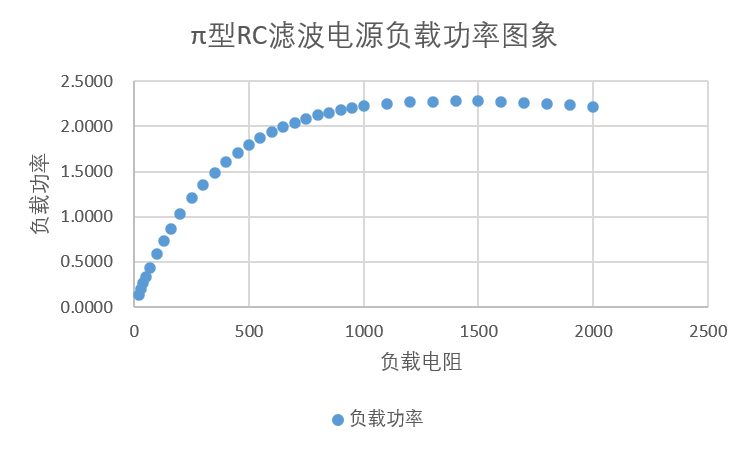
\includegraphics[scale=0.6]{pigl.png}

    \end{minipage}
    \begin{minipage}[t]{0.48\textwidth}
        \centering
        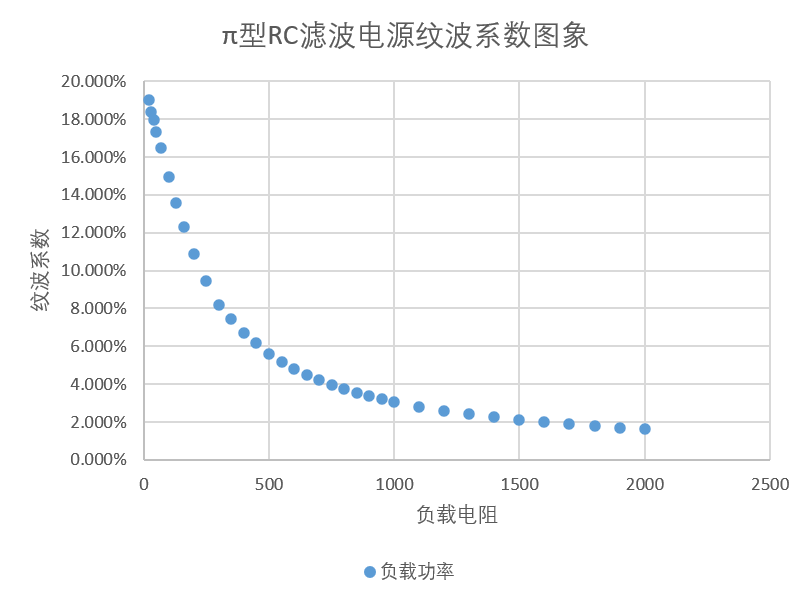
\includegraphics[scale=0.5]{piwb.png}
    \end{minipage}
\end{figure}
\begin{figure}[tbp]
    \centering
    \begin{minipage}[t]{0.48\textwidth}
        \centering
        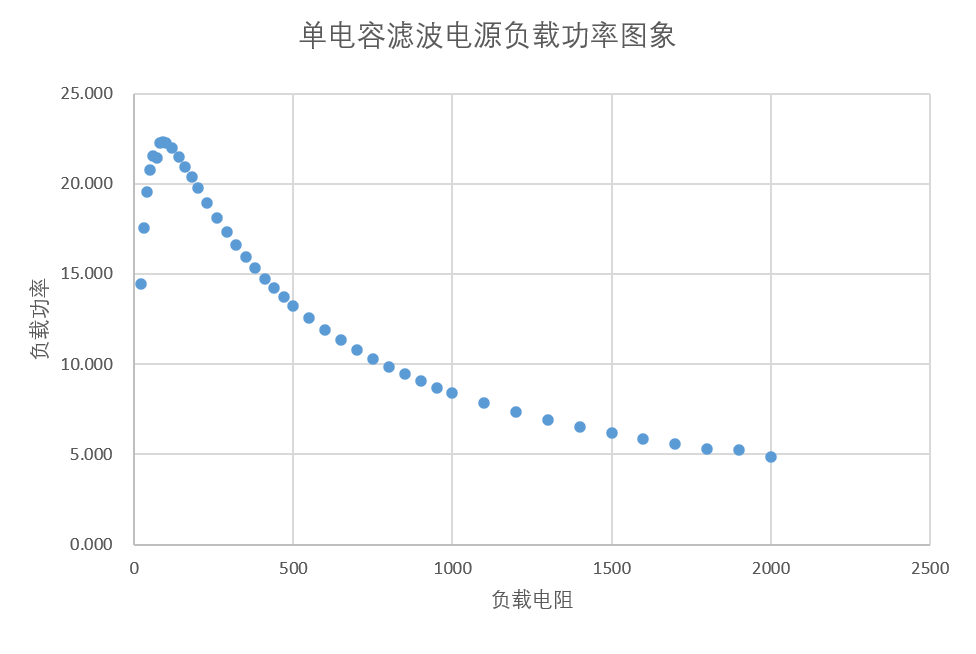
\includegraphics[scale=0.5]{ddrgl.png}

    \end{minipage}
    \begin{minipage}[t]{0.48\textwidth}
        \centering
        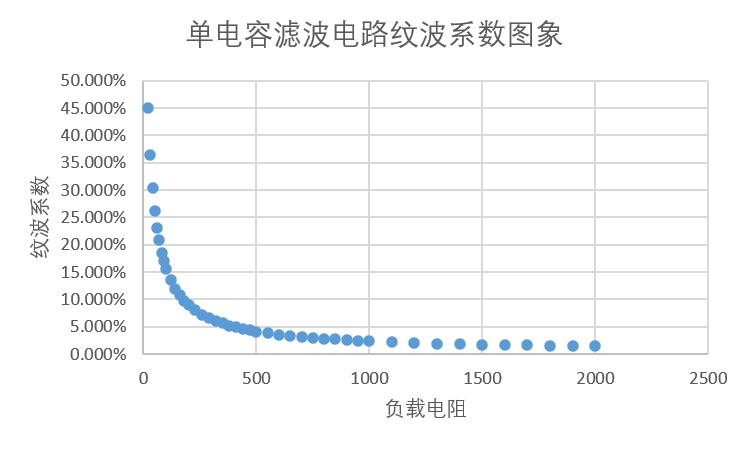
\includegraphics[scale=0.75]{ddrwb.png}
    \end{minipage}
\end{figure}

由图可见,单电容电路滤波的功率最大值出现在负载约等于90$\Omega$处;$\pi$型 RC 电路滤波的功率最大
值出现在负载约等于1.4$k\Omega$处。纹波系数都随负载增加而降低,单电容电源在负载较低时纹波系数较大,但随着负载增加迅速降低。
\newpage
\subsection*{非线性内阻电源开路电压和短路电流的测定}
开路电压 $V=\SI{1.6005}{V}$, 短路电流 $I=\SI{5.8}{mA}$

由此计算得内阻\[R=\frac{V}{I}=\frac{1.6005}{5.8\times 10^{-3}}\approx280\Omega\]
\section*{误差分析}
不同负载下纹波系数和功率的测量实验的主要误差在于万用表读数不太稳定,采集某些数据点时后几位不稳定,记录时
人为选取了一个数据,具有较大偶然性。

非线性内阻电源开路电压和短路电流的测定实验的主要误差在于读取检流计零刻度线处有一定的偏差,变阻器较难控制使得检流计维持在零刻度。
此外,毫安表测量精度有限。

\section*{思考题}
简述单大电容和小电容 π 型滤波的优劣。

    大电容优势:能提供更大的电压、功率。
    
    大电容劣势:当交流电频率较低时纹波系数大,电流不稳定。

    小电容滤波的优劣与之相对应。


\end{document}